% ! TeX program = lualatex
\documentclass[a4paper,11pt]{article} 
% packages
\usepackage{censor}
\StopCensoring
\usepackage{fontspec}
\setmainfont{EB Garamond}
% for tironian et fallback
% % \directlua{luaotfload.add_fallback
% % ("emojifallback",
% %      {"Noto Serif:mode=harf"}
% % )}
% % \setmainfont{EB Garamond}[RawFeature={fallback=emojifallback}]

\setmonofont[Scale=MatchLowercase]{Deja Vu Sans Mono}
\usepackage[a4paper,left=2cm,right=2cm,top=\dimexpr15mm+1.5\baselineskip,bottom=2cm]{geometry}
\setlength{\parindent}{0pt}

\usepackage{fancyhdr}       % Headers and footers 
\fancyhead[R]{\normalfont \leftmark}
\fancyhead[L]{}
\pagestyle{fancy}

\usepackage{microtype}      % Slightly tweak font spacing for aesthetics
\usepackage[english]{babel} % Language hyphenation and typographical rules
\usepackage{xcolor}
\definecolor{linkblue}{RGB}{0, 64, 128}
\usepackage[final, colorlinks = false, urlcolor = linkblue]{hyperref} 
% \newcommand{\secref}[1]{\textbf{§~\nameref{#1}}}
\newcommand{\secref}[1]{\textbf{§\ref{#1}~\nameref{#1}}}

\usepackage{amsmath}
\usepackage[most]{tcolorbox}
\usepackage{changepage}     % adjust margins on the fly
\usepackage{amsmath,amssymb}

\usepackage{minted}
\usemintedstyle{algol_nu}

\usepackage{pgfplots}
\pgfplotsset{width=\textwidth,compat=1.9}

\usepackage{caption}
\newenvironment{code}{\captionsetup{type=listing}}{}
\captionsetup[listing]{skip=0pt}
\setlength{\abovecaptionskip}{5pt}
\setlength{\belowcaptionskip}{5pt}

\usepackage[yyyymmdd]{datetime}
\renewcommand{\dateseparator}{--}

\usepackage{enumitem}

\usepackage{titlesec}

\author{Andrew Hayes}

\begin{document}
\begin{titlepage}
    \begin{center}
        \hrule
        \vspace*{0.6cm}
        \Huge \textsc{cs4423}
        \vspace*{0.6cm}
        \hrule
        \LARGE
       \vspace{0.5cm}
       Networks
       \vspace{0.5cm}
       \hrule

       \vfill

       \hrule
        \begin{minipage}{0.495\textwidth} 
            \vspace{0.4em}
            \raggedright
            \normalsize 
            \begin{tabular}{@{}l l}
                Name: & Andrew Hayes \\
                Student ID: & 21321503 \\
                E-mail: & \href{mailto://a.hayes18@universityofgalway.ie}{a.hayes18@universityofgalway.ie} \\
            \end{tabular}
        \end{minipage}
        \begin{minipage}{0.495\textwidth} 
            \raggedleft
            \vspace*{0.8cm}
            \Large
            \today
            \vspace*{0.6cm}
        \end{minipage}
        \medskip\hrule 
    \end{center}
\end{titlepage}

\pagenumbering{roman}
\newpage
\tableofcontents
\newpage
\setcounter{page}{1}
\pagenumbering{arabic}

\section{Introduction}
\textbf{CS4423 Networks} is a Semester 2 module on \textbf{Network Science}.
Modern societies are in many ways highly connected.
Certain aspects of this phenomenon are frequently described as \textbf{networks}.
CS4423 is an introduction to this emerging interdisciplinary subject.
We'll cover several major topics in this module, including:
\begin{itemize}
    \item   Graphs \& Graph Theory,  and how they relate to networks;
    \item   Representations of networks, including as matrices;
    \item   Computing with networks, using \mintinline{python}{networkx} in Python;
    \item   Centrality measures;
    \item   Random graphs;
    \item   Small worlds;
    \item   Models of growing graphs;
\end{itemize}

Lecture notes \& assignments will come in the form of Jupyter notebooks, which allows us to include interactive Python code with the text.

\subsection{Lecturer Contact Information}
\begin{itemize}
    \item   Name: Dr Niall Madden.
    \item   School of Mathematical \& Statistical Sciences, University of Galway.
    \item   Office: Room ADB-1013, Arás de Brún.
    \item   E-mail: \href{mailto://niall.madden@universityofgalway.ie}{niall.madden@universityofgalway.ie}.
    \item   Website: \url{https://www.niallmadden.ie}
\end{itemize}

\subsection{Exam Information}
First year lecturing, should be similar to old exam papers.
Only looked at the past 2 years or so.

\subsection{Schedule}
Tentative schedule for labs / tutorials:
\begin{itemize}
    \item   Tuesday at 16:00 in AC215;
    \item   Wednesday at 10:00 in CA116a.
\end{itemize}

There will be some practicals during the semester: Week 3 ``Introduction to Python \& Jupyter'' sessions, later weeks help with assignments, preparations for exam, etc.

\subsection{Assessment}
\begin{itemize}
    \item   Two homework assignments.
            Tentative deadlines: Weeks 5 \& 10.
            Each contribute 10\% each to the final grade.

    \item   One in-class test.
            Probably Week 7 (depending on FYP deadlines).
            Contributes 10\% to the final grade.

    \item   Final exam: 70\%.
\end{itemize}

\subsection{Introduction to Networks}
Newman (for example) broadly divides the most commonly studied real-world networks into four classes:
\begin{enumerate}
    \item   \textbf{Technological networks:} rely on physical infrastructure.
            In many cases, this infrastructure has been built over many decades and forms part of the backbone of modern societies, including roads \& other transportation networks, power grids, and communications networks.

    \item   \textbf{Social networks:} the vertices of a social network are people (or, at leasts, User IDs), with edges representing some sort of \textbf{social interaction}.
            In sociology, the vertices are often called \textbf{actors}, and the edges are called \textbf{ties}.
            Social networks are not just online: sociologists have studied social networks long before people started exhibiting their relations to others online.
            Traditionally, data about the structure of social networks have been compiled by interviewing the people involved.

    \item   \textbf{Information networks:} consist of \textbf{data items} which are linked to each other in some way.
            Examples include relational databases.
            Sets of information (like scientific publications) have been linking to each other (e.g., through citations) long before computers were invented, although links in digital form are easier to follow.
            \\\\
            The \textbf{WWW} is probably the most widespread \& best-known example of an information network.
            Its nodes are \textbf{web pages} containing information in form of text \& pictures, and its edges are the \textbf{hyperlinks}, allowing us to surf or navigate from page to page.
            Hyperlinks run in one direction only, from the page that contains the hyperlink to the page that is referenced.
            Therefore, the WWW is a \textbf{directed network}, a graph where each edge has a direction.

    \item   \textbf{Biological networks:}
            \begin{itemize}
                \item   \textbf{Biochemical networks} represent molecular-level patterns of interaction \& control mechanisms in the biological cell, including metabolic networks, protein-protein interaction networks, \& genetic regulatory networks.

                \item   A \textbf{neural network} can be represented as a set of vertices, the neurons, connected by two types of directed edges, one for excitatory inputs and one for inhibitory inputs.
                        (Not to be confused with an artificial neural network).

                \item   \textbf{Ecological networks} are networks of ecological interactions between species.
            \end{itemize}
\end{enumerate}

In each case, a network connects parts of a system (\textbf{nodes}) by some means (\textbf{links}).
Different techniques are used to display, discover, \& measure the structure in each example.
\\\\
In its simplest form, a \textbf{network} is just a collection of points (called \textbf{vertices} or \textbf{nodes}), some of which are joined in pairs (called \textbf{edges}  or \textbf{links}).
Many systems of interest are composed of individual parts that are in some way linked together: such systems can be regarded as networks, and thinking about them in this way can often lead to new \& useful insights.
\\\\
\textbf{Network science} studies the patterns of connections between the components of a system.
Naturally, the structure of the networks can have a big impact on the behaviour of the system.
A \textbf{network} is a simplified representation of a complex system by vertices \& edges.
The scientific study of networks is an interdisciplinary undertaking that combines ideas from mathematics, computer science, physics, the social sciences, \& biology.
Between these scientific fields, many tools have been developed for analysing, modeling, \& understanding networks.

\subsubsection{Network Measures}
\textbf{Centrality} is an example of a useful \& important type of network measure; it is concerned with the question of how important a particular vertex or edge is in a networked system.
Different concepts have been proposed to capture mathematically what it means to be central.
For example, a simple measure of the centrality of a vertex is its \textbf{degree}, that is, the number of edges it is part of (or, equivalently, the number of vertices it is adjacent to).
Applications of centrality include determining which entities in a social network have the most influence, or which links in a power grid are most vulnerable.
\\\\
Which measurements \& calculations give meaningful answers for a particular system depends of course on the specific nature of the system and the questions one wants to ask. 

\subsubsection{Network Concepts}
Another interesting network concept is the \textbf{small-world effect}, which is concerned with the question of how far apart two randomly chosen points in a network typically are.
Here, \textbf{distance} is usually measured by the number of edges one would need to cross over when travelling along a \textbf{path} from one vertex to another.
In real-world social networks, the distance between people tends to be rather small.

\section{Graphs}
A \textbf{graph} can serve as a mathematical model of a network.
Later, we will use the \mintinline{python}{networkx} package to work with examples of graphs \& networks.

\subsection{Example: The Internet (circa 1970)}
\begin{figure}[H]
    \centering
    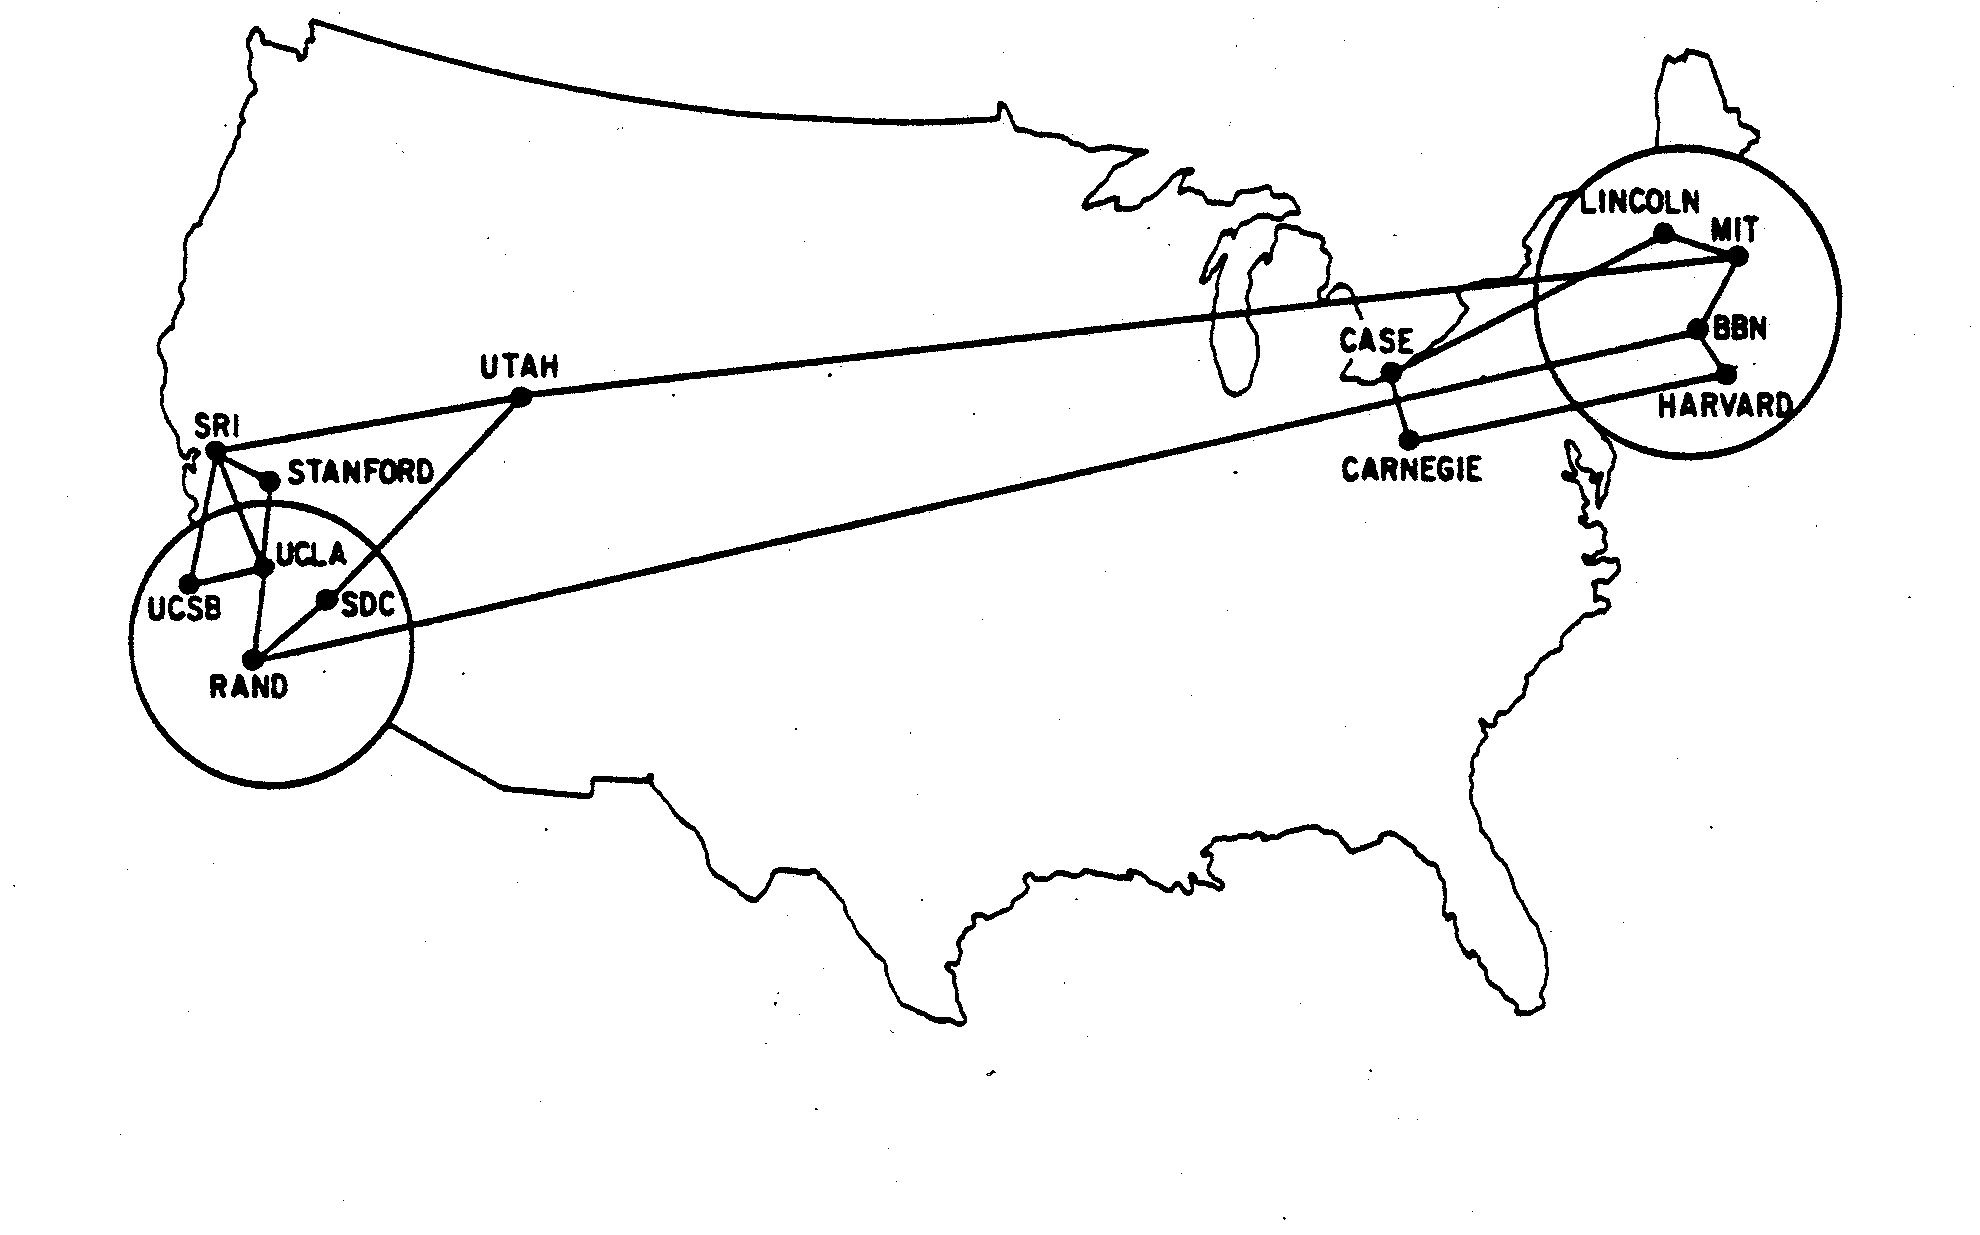
\includegraphics[width=0.7\textwidth]{./images/f7dec1970.jpg}
    \caption{
        The Internet (more precisely, ARPANET) in December 1970.
        Nodes are computers, connected by a link if they can directly communicate with each other.
        At the time, only 13 computers participated in that network.
    }
\end{figure}

\begin{code}
\begin{minted}[linenos, breaklines, frame=single]{text}
UCSB SRI UCLA
SRI UCLA STAN UTAH
UCLA STAN RAND
UTAH SDC MIT
RAND SDC BBN
MIT BBN LINC
BBN HARV
LINC CASE
HARV CARN
CASE CARN
\end{minted}
\caption{\texttt{arpa.adj}}
\end{code}

The following \textbf{diagram}, built from the adjacencies in \verb|arpa.adj|, contains the same information as in the above figure, without the distracting details of US geography;
this is actually an important point, as networks only reflect the \textbf{topology} of the object being studied.

\begin{code}
\begin{minted}[linenos, breaklines, frame=single]{python}
H = nx.read_adjlist("../data/arpa.adj")
opts = { "with_labels": True, "node_color": 'y' }
nx.draw(H, **opts)
\end{minted}
\caption{\texttt{arpa.adj}}
\end{code}

\begin{figure}[H]
    \centering
    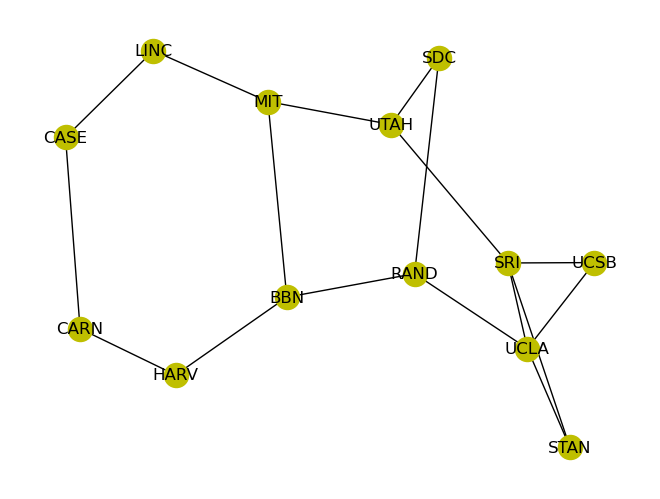
\includegraphics[width=0.7\textwidth]{./images/qwe_download.png}
    \caption{ The ARPA Network as a Graph }
\end{figure}

\subsection{Simple Graphs}
A \textbf{simple graph} is a pair $G = (X,E)$ consisting of a finite set $X$ of objects called \textit{nodes}, \textit{vertices}, or \textit{points} and a set of \textit{links} or \textit{edges} $E$ which are each a set of two different vertices. 
\begin{itemize}
    \item   We can also write $E \subseteq \binom{X}{2}$, where $\binom{X}{2}$ ($X$ \textit{choose} 2) is the set of all $2$-element subsets of $X$.
    \item   The \textbf{order} of the graph $G$ is denoted as $n = |X|$, where $n$ is the number of vertices in the graph.
    \item   The \textbf{size} of the graph is denoted as $m = |E|$, where $m$ is the number of edges in the graph.
            Naturally, $m \leq \binom{n}{2}$.
\end{itemize}

\subsection{Subgraphs \& Induced Subgraphs}
Given $G = (X,E)$, a \textbf{subgraph} of $G$ is $H=(Y, E_H)$ with $Y \subseteq X$ and $E_H \subseteq  E \cap \binom{Y}{s}$;
therefore, all the nodes in $H$ are also in $G$ and any edge in $H$ was also in $G$, and is incident only to vertices in $Y$.
\\\\
One of the most important subgraphs of $G$ is the \textbf{induced subgraph} on $Y \subseteq X$: $H = (Y, E \cap \binom{Y}{2})$;
that is, given a subset $Y$ of $X$, we include all possible edges from the original graph $G$ too.
Each node has a list of \textbf{neighbours} which are the nodes it is directly connected to by an edge of the graph.

\subsection{Important Graphs}
The \textbf{complete graph} on a vertex set $X$ is the graph with edge set $\binom{X}{2}$.
For example, if $X = \{0,1,2,3 \}$, then $E = \{01,02,03,12,13,23\}$
\\\\
The \textbf{Petersen graph} is a graph on 10 vertices with 15 edges.
It can be constructed as the complement of the line graph of the complete graph $K_5$, that is, as the graph with the vertex set $X = \binom{ \{0,1,2,3,4\} }{2}$ (the edge set of $K_5$) and with an edge between $x,y \in X$ whenever $x \cap y = \emptyset$.
\\\\
A graph is \textbf{bipartite} if we can divide the node set $X$ into two subsets $X_1$ and $X_2$ such that:
\begin{itemize}
    \item   $X_1 \cap X_2 = \emptyset$  (the sets have no edge in common);
    \item   $X_1 \cup X_2 = X$.
\end{itemize}

For any edge $(u_1, u_2)$, we have $u_1 \in X_1$ and $u_2 \in X_2$; that is, we only ever have edges between nodes from different sets.
Such graphs are very common in Network Science, where nodes in the network represent two different types of entities; for example, we might have a graph wherein nodes represent students and modules, with edges between students and modules they were enrolled in, often called an \textbf{affiliation network}.
\\\\
A \textbf{complete bipartite graph} is a particular bipartite graph wherein there is an edge between every node in $X_1$ and every node in $X_2$.
Such graphs are denoted $K_{m,n}$, where $|X_1| = m$ and $|X_2|=n$.
\\\\
The \textbf{path graph} with $n$ nodes, denoted $P_n$, is a graph where two nodes have degree 1, and the other $n-2$ have degree 2.
\\\\
The \textbf{cycle graph} on $n \geq 3$ nodes, denoted $C_n$ (slightly informally) is formed by adding an edge between the two nodes of degree 1 in a path graph.

\subsection{New Graphs from Old}
The \textbf{complement} of a graph $G$ is a graph $H$ with the same nodes as $G$ but each pair of nodes in $H$ are adjacent if and only if they are \textit{not adjacent} in $G$.
The complement of a complete graph is an empty graph.
\\\\
A graph $G$ can be thought of as being made from ``things'' that have connection to each other: the ``things'' are nodes, and their connections are represented by an edge.
However, we can also think of edges as ``things'' that are connected to any other edge with which they share a vertex in common.
This leads to the idea of a line graph:
the \textbf{line graph} of a graph $G$, denoted $L(G)$ is the graph where every node in $L(G)$ corresponds to an edge in $G$, and for every pair of edges in $G$ that share a node, $L(G)$ has an edge between their corresponding nodes.

\section{Matrices of Graphs}
There are various was to represent a graph, including the node set, the edge set, or a drawing of the graph;
one of the most useful representations of a graph for computational purposes is as a \textbf{matrix}; the three most important matrix representations are:
\begin{itemize}
    \item   The \textbf{adjacency matrix} (most important);
    \item   The \textbf{incidence matrix} (has its uses);
    \item   The \textbf{graph Laplacian} (the coolest).
\end{itemize}

\subsection{Adjacency Matrices}
The \textbf{adjacency matrix} of a graph $G$ of order $n$ is a square $n \times n$ matrix $A = (a_{i,j})$ with rows \& columns corresponding to the nodes of the graph, that is, we number the nodes $1, 2, \dots, n$.
Then, $A$ is given by:
\begin{align*}
    a_{i,j} =
    \begin{cases}
        1 & \text{if nodes } i \text{ and } j \text{ are joined by an edge,} \\
        0 & \text{otherwise}
    \end{cases}
\end{align*}

Put another way, $a_{i,j}$ is the number of edges between node $i$ and node $j$.
Properties of adjacency matrices include:
\begin{itemize}
    \item   $\sum^N_{i=1} \sum^N_{j=1} a_{i,j} = \sum_{u \in X}\text{deg}(u)$ where $\text{deg}(u)$ is the degree of $u$.
    \item   All graphs that we've seen hitherto are \textit{undirected}: for all such graphs, $A$ is symmetric.
            $A = A^T$ and, equivalently, $a_{i,j} = a{j,i}$.
    \item   $a_{i,i} = 0$ for all $i$.
    \item   In real-world examples, $A$ is usually \textbf{sparse} which means that $\sum^N_{i=1} \sum^N_{j=1} a_{i,j} \ll n^2$, that is, the vast majority of the entries are zero.
            Sparse matrices have huge importance in computational linear algebra: an important idea is that is much more efficient to just store the location of the non-zero entities in a sparse matrix.
\end{itemize}

Any matrix $M = (m_{i,j})$ with the properties that all entries are zero or one and that the diagonal entries are zero (i.e., $m_{i,j}=0$) is an adjacency matrix of \textit{some} graph (as long as we don't mind too much about node labels).
In a sense, every square matrix defines a graph if:
\begin{itemize}
    \item   We allow loops (an edge between a node and itself).
    \item   Every edge has a weight: this is equivalent to the case for our more typical graphs that every potential edge is weighted 0 (is not in the edge set)  or 1 (is in the edge set).
    \item    There are two edges between each node (one in each direction) and they can have different weights.
\end{itemize}

\subsubsection{Examples of Adjacency Matrices}
Let $G = G(X,E)$ be the graph with $X = \{a,b,c,d,e\}$ nodes and edges $\{a \leftrightarrow b, b \leftrightarrow c, b \leftrightarrow d, c \leftrightarrow d, d \leftrightarrow e \}$.
Then:
\begin{align*}
    A =
    \begin{pmatrix}
        0 & 1 & 0 & 0 & 0 \\
        1 & 0 & 1 & 1 & 0 \\
        0 & 1 & 0 & 1 & 0 \\
        0 & 1 & 1 & 0 & 1 \\
        0 & 0 & 0 & 1 & 0 \\
    \end{pmatrix}
\end{align*}

The adjacency matrix of $K_4$ is:
\begin{align*}
    A =
    \begin{pmatrix}
        0 & 1 & 1 & 1 \\
        1 & 0 & 1 & 1 \\
        1 & 1 & 0 & 1 \\
        1 & 1 & 1 & 0 \\
    \end{pmatrix}
\end{align*}

\subsection{Degree}
The \textbf{degree} of a node in a simple graph is the number of nodes to which it is adjacent, i.e., its number of neighbours.
For a node $v$ we denote this number $\text{deg}(v)$.
The degree of a node can serve as a (simple) measure of the importance of a node in a network.
Recall that one of the basic properties of an adjacency matrix is $\sum^n_{i=1} \sum^n_{j=1} a_{i,j} = \sum_{u \in X} \text{deg}(u)$, where $\text{deg}(u)$ is the degree of $u$ and $n$ is the order of the graph;
this relates to a (crude) measure of how connected a network is: the \textbf{average degree}:
\begin{align*}
    \text{Average degree} = \frac{1}{n} \sum_{u \in X} \text{deg}(u) = \frac{1}{n}\sum^n_{i,j} a_{i,j}
\end{align*}
However, if the size of the network (the number of edges) is $m$, then the total sum of degrees is $2m$ (since each edge contributes to the degree count of two nodes), meaning that the average degree is $\frac{2m}{n}$.

\subsection{Walks}
A \textbf{walk} in a graph is a series of edges (perhaps with some repeated) $\{ u_1 \leftrightarrow v_1, u_2 \leftrightarrow u_2, \dots, u_p \leftrightarrow v_p\}$ with the property that $v_i = u_{i+1}$.
If $v_p = u_1$, then it is a \textbf{closed walk}.
The \textbf{length} of a walk is the number of edges in it.
\\\\
Adjacency matrices can be used to enumerate the number of walks of a given length between a pair of vertices.
Obviously, $a_{i,j}$ is the number of walks of length 1 between node $i$ and node $j$.
We can extract that information for node $j$ by computing the product of $A$ and $e_j$ (column $j$of the identity matrix).

\section{Connectivity \& Permutations}
To start, let's decide on our notation:
\begin{itemize}
    \item   If we write $A = (a_{i,j})$, we mean that $A$ is a matrix and $a_{i,j}$ is its entry row $i$, column $j$.
    \item   We also write such entries as $(A)_{i,j}$;
            the reason for this slightly different notation is to allow us to write, for example, $(A^2)_{i,j}$ is the entry in row $i$, column $j$ of $B = A^2$.
    \item   The \textbf{trace} of a matrix is the sum of its diagonal entries, that is, $\text{tr}(A) = \sum^n_{i=1}a_{i,i}$. (Very standard).
    \item   When we write $A > 0$, we mean that all entries of $A$ are positive.
\end{itemize}

Recall that the \textbf{adjacency matrix} of a graph $G$ of order $N$ is a square $n \times n$ matrix $A = (a_{i,j})$ with rows and columns corresponding to the nodes of the graph.
$a_{i,j}$ is set to be the number of edges between nodes $i$ and $j$.
We learned previously that:
\begin{itemize}
    \item   If $e_j$ is the $j^\text{th}$ column of the 
\end{itemize}







\end{document}
